\documentclass[PREyA.tex]{subfiles}

\usepackage{tikz}
\usetikzlibrary{automata,positioning}
\providecommand{\abs}[1]{\left\lvert#1\right\rvert}
\begin{document}

\chapter{Cadenas de Markov en tiempo continuo}
\section{Introducción}
\begin{defi}
Se dice que una cadena en tiempo continuo es de Markov si verifica la propiedad de Markov, es decir, si $\forall n \geq 2$ $\forall 0\leq t_1 < \dotsc < t_n$ y $\forall i_1,\dotsc,i_n\in S$ se verifica
$$
P[X_{t_n} = i_n \mid X_{t_1}=i_1,\dotsc,X_{t_{n-1}}=i_{n-1}] = P[X_{t_n} = i_n \mid X_{t_{n-1}} = i_{n-1}]
$$
\end{defi}
\begin{defi}
A los valores $i_1,\dotsc,i_{n-1}$ se les denomina \textbf{historia} y, en particular, $i_{n-1}$ es el \textbf{pasado inmediato}.
\end{defi}
\begin{example}
El proceso de Poisson verifica la propiedad markoviana. Se deduce trivialmente a partir de incrementos independientes.
\end{example}
\begin{defi}
Podemos considerar $p_{ij}^{(s,t)}$ a la probabilidad de que el proceso en el instante $t$ esté en $j$ condicionado a que en el instante $s$ estaba en $i$, es decir,
$$
p_{ij}^{(s,t)} = P[X_t =j \mid X_s = i]
$$
Luego podemos considerar $P_{st} = (p_{ij}^{(s,t)})$ con $i,j \in S$ y para $0\leq s \leq t$.
\end{defi}
\begin{nota}
Supondremos en adelante que se verifica la propiedad de homogeneidad en el tiempo, es decir, que las $p_{ij}^{(s,t)}$ son funciones de la diferencia en el tiempo $t-s$. 
\end{nota}
\begin{nota}
Bajo la asunción anterior podemos escribir simplemente $P_t = (p_{ij}^{(0,t)})$, pues
$$
P[X(t+s)=j \mid X(s)=i] = P[X(t)=j\mid X(0)=i]
$$
\end{nota}
\newpage
\begin{prop}
Se verifican las siguientes propiedades
\begin{itemize}
\item $P_0 = I_{|S|\times |S|}$.
\item $P_t$ es una matriz estocástica.
\item Verifica las ecuaciones de Chapman Kolmogorov, es decir
$$
P_{t+s}=P_tP_s \quad \forall s,t\geq 0
$$
\end{itemize}
\end{prop}
\begin{dem} Tenemos
\begin{itemize}
\item $p_{ij}(0) = P[X(0)=j\mid X(0)=i]$.
\item Sumamos directamente
\begin{align*}
1 &= P[X(t)\in S \mid X(0)=i] \\
&= \sum_{j \in S} P[X(t)=j \mid X(0)=i]\\
&=\sum_{j\in S} p_{ij}(t)
\end{align*}
\item 
\begin{align*}
p_{ij}(t+s) &= P[X(t+s) =j \mid X(0)=i]\\
& = P[X(t+s)=j, X(t)\in S \mid X(0)=i]\\
&=\sum_{k \in S} P[X(t+s)=j, X(t)=k \mid X(0)=i]\\
&=\sum_{k\in S} P[X(t) = k  \mid X(0)=i] P[X(t+s) = j \mid X(0)=i, X(t)=k]\\
&=\sum_{k\in S} P[X(t) = k  \mid X(0)=i] P[X(t+s) = j \mid  X(t)=k]\\
&=\sum_{k\in S} p_{ik}(t) P[X(s) = i \mid  X(0)=k]\\
&=\sum_{k\in S} p_{ik}(t) p_{kj}(s) 
\end{align*}
Por tanto, $P_{t+s} = P_t P_s$.
\end{itemize}

\end{dem}
\begin{prop}
El conjunto $\{P_t\}_{t\geq 0}$ tiene estructura de semigrupo con la operación producto.
\end{prop}
\begin{nota}
Vamos a suponer por simplicidad que todos los semigrupos son standar, es decir, 
$$
\lim_{t\to0} P_t = I
$$
\end{nota}

\begin{nota}
Describir una cadena de Markov a partir de sus matrices de probabilidad y el estado inicial puede ser costoso en la práctica.
\end{nota}
\begin{defi}
Definimos la matriz de generadores siempre que tenga sentido
$$
G:= \lim_{h\to 0^+} \frac{P_h -I }{h} 
$$
\end{defi}
\begin{nota}
Otra forma de expresar la idea anterior es
\begin{align*}
g_{ij}h &= p_{ij}(h) - o(h)\\
g_{ii}h &= p_{ii}(h) - o(h) -1
\end{align*}
O, equivalentemente
\begin{align*}
p_{ij}(h) &= g_{ij}h + o(h)\\
p_{ii}(h) &= 1+ g_{ii}h + o(h) 
\end{align*}
\end{nota}
\begin{prop}
Bajo la hipótesis de que los semigrupos son standar, se tiene que
$$
G= (p_{ij}'(0))
$$
\end{prop}
\begin{prop}
Se verifican las siguientes propiedades
\begin{enumerate}
\item $g_{ij}\geq 0$ $\forall i \neq j$
\item $g_{ii} \leq 0$ 
\item $\sum_{j} g_{ij} = 0$ $\forall i$
\end{enumerate}
\end{prop}
\begin{dem}
\begin{enumerate}
\item[]
\item Sabemos que $p_{ij}(h)>0$ $\forall h$, luego
$$
g_{ij}=\lim_{h\to0^+}\frac{p_{ij}(h)}{h}\geq 0
$$
\item Análogamente
$$
g_{ij}=\lim_{h\to0^+}\frac{p_{ij}(h)}{h}\leq 0
$$
\item Dado que $P_t$ es una matriz estocástica, se verifica
$$
\sum_{j}p_{ij}(t)=1
$$
Derivando y haciendo $t\to 0$ obtenemos
$$
0 = \sum_j p'_{ij}(t)_{t\to 0} = \sum_j p'_{ij}(0) = \sum_j g_{ij}
$$
\end{enumerate}
\end{dem}
\begin{prop}[Ecuaciones backward y forward]
Sea $P_0 =I$. Entonces $P_t' = GP_t = P_tG$.
\end{prop}
\begin{dem}
La demostración se tiene directamente
$$
P_t' = \lim_{h\to0}\frac{P_{t+h}-P_t}{h} \lim_{h\to0}\frac{P_{h}P_t-P_t}{h} = \lim_{h\to0}\frac{(P_h-I)P_t}{h}=G P_t
$$
La otra igualdad es análoga.
\end{dem}
\begin{nota}
Notemos que, en particular, $P_t$ verifica la ecuación diferencial matricial $y=cy'$. Por tanto, $P_t = \exp(Gt)$, donde para cualquier matriz $A$ cuadrada
$$
\exp(A)=\sum_{i=0}^\infty \frac{A^n}{n!}
$$
Esta función verifica la siguiente propiedad: Si $A$ y $B$ conmutan ($AB=BA$), entonces $\exp(A+B)=\exp(A)\exp(B)$. Si $A$ se descompone en su forma canónica de Jordan $PJP^{-1}$, entonces se verifica $\exp(A)=P\exp(J)P^{-1}$.
\end{nota}
\begin{prop}[Interpretación de $G$] 
\begin{itemize}
\item[]
\item Elementos diagonales $g_{ii}$. Sea $T_i$ el tiempo de permanencia en un estado $i$. Entonces $T_i \sim Exp(-g_ii)$
\item Elementos extradiagonales $g_{ij}$ $i\neq j$.  La probabilidad de saltar al estado $j$ suponiendo que estamos en $i$ es $-g_{ij}/g_{ii}$.
\end{itemize}
\end{prop}
\begin{dem}
Por la homogeneidad en el tiempo podemos suponer que estamos en el instante $t=0$. Para la primera part vamos a calcular el complementario la función de distribución
\begin{align*}
P[T_i > t] &\approx P[X_{i/N} =i \colon \forall i = 1,\dotsc tN, \forall N \mid X_0 = i]\\
&= \prod_{i=1}^{Nt} P[X_{i/N}=i\mid X_{(i-1)/N}=i]\\
&= p_{ii}\left(\frac{1}{N}\right)^{tN} \\
&= \left(1+\frac{g_{ii}}{N}+o(1/N)\right)^{tN} \longrightarrow e^{-g_{ii} t}
\end{align*}
Para la segunda parte consideramos
\begin{align*}
P[N(t+h) = j \mid N(t)=i \text{ y hay salto}] &= \frac{P[N(t+h) = j, N(t)=i \text{ y hay salto}]}{P[N(t)=i \text{ y hay salto}]}\\
&=\frac{P[N(t)=i]P[N(t+h)=j\mid N(t)=i,\;i\neq j}{P[N(t)=i]P[\text{Hay salto}\mid N(t)=i]}\\
&=\frac{P[N(t)=i]p_{ij}(h)}{P[N(t)=i]\sum_{k\neq i} P[N(t+h)=k\mid N(t)=i]}\\
&=\frac{p_{ij}(h)}{\sum_{k\neq i} p_{ik}(h)}= \frac{g_{ij}h+o(h)}{\sum_{k\neq i} g_{ik}h+o(h)}\\
&\overset{h\to 0}{\approx} -\frac{g_{ij}}{g_{ii}}
\end{align*}
\end{dem} 
\begin{nota}
La representación de una cadena de Markov en tiempo continuo a través de un grafo se realiza escribiendo sobre las flechas los elementos de $G$, salvo los loops que no se escriben. 

Por ejemplo, sea una cadena de Markov dada por la matriz
$$
G= 
\begin{pmatrix}
-a & a\\
b & -b
\end{pmatrix}
$$
Entonces el grafo asociado es
\begin{center}
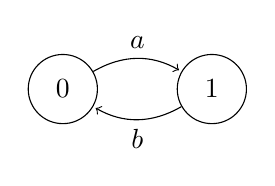
\begin{tikzpicture}
	% Draw the states
	\node[state]             (1) {$0$};
	\node[state, right=of 1] (2) {$1$};
    % Connect the states with arrows
	\draw[every loop]
		(1) edge[bend left, auto=left] node {$a$} (2)
		(2) edge[bend left, auto=left] 	   node {$b$} (1);
\end{tikzpicture}
\end{center}
\end{nota}

\section{Cadena de Markov en tiempo discreto}
Sabemos que en $t_0$ $X(0)$ es el primer valor de la cadena. Entonces podemos definir 
$$
W_1 = \sup\{t>0 \mid X(t)=X(0)\}
$$
y se sigue
$$
W_j = \sup\{t>0\mid X(t) = X(W_{j-1})\}
$$
Definimos para un nuevo proceso discreto $Y_n$ dado por $Y_n = X(W_n)$. Este es proceso es una cadena de Markov de parámetro discreto. Además su matriz de transición es una matriz con diagonal nula y el resto de elementos son $-g_{ij}/g_{ii}$. 
\section{Distribuciones condicionadas}
\begin{defi}
Se dice que una distribución de probabilidad $\pi$ con $\pi_i \geq 0$ y $\sum_i \pi_i = 1$ es una distribución estacionaria si verifica que
$$
\pi = \pi P_t \quad \forall t
$$
En caso de existir, no depende del tiempo. Su cálculo puede ser complicado.
\end{defi}
\begin{prop}
Una distribución $\pi$ es estacionaria si y solo si $\pi G = 0$.
\end{prop}
\begin{dem}
Si $\pi$ es estacionaria, entonces $\pi P_t = \pi$. Por tanto
$$
\pi G = \pi \lim_{t\to 0} \frac{P_t - I}{t} = \lim_{t\to 0} \frac{\pi P_t - \pi}{t} = \lim_{t\to 0} 0 = 0
$$
Si $\pi G = 0$, entonces considerems $P_t = \exp(tG) = \sum_{k=0}^\infty (tG)^k/k!$. Entonces
$$
\pi P_t = \pi  \sum_{k=0}^\infty (tG)^k/k! = \pi +  \sum_{k=1}^\infty t^k\pi G^k/k! = \pi
$$
\end{dem}


\begin{theorem}
Sean $X_1,\dotsc,X_n$ independientes y $X_i \sim Exp(\lambda_i)$, $i=1,\dotsc,n$. Entonces
\begin{itemize}
\item 
$$
\min_{i=1,\dotsc,n} X_i  \sim Exp\left(\sum_{i=1}^n\lambda_i\right)
$$
\item
$$
P\left[\min_{i=1,\dotsc,n} X_i = X_j\right] = \frac{\lambda_j}{\sum_{i=1}^n \lambda_j}
$$
\end{itemize}
\end{theorem}
\begin{nota}
Si ponemos a competir dos temporizadores aleatorios, de manera que gana el que salte antes, entonces $Z_i \sim Exp(\lambda_i)$ $i=1,2$. Aplicando el teorema anterior, la probabilidad de que gane $X_i$ es $\lambda_i / (\lambda_1 + \lambda_2)$.
\end{nota}

\begin{prop}
Consideremos $\rho_k(t)= P[X(t)=k]$. Sea además $\rho_t = (\rho_i(t))_{i \in \mathbb{N}\cup\{0\}}$. Entonces
$$
\rho_t'=\rho_t G
$$
\end{prop}
\begin{dem}
Sabemos que $\rho_t = \rho_0 P_t$ y que la ecuación forward que verifica $P_t$ es $P_t' = P_t G$. Entonces
\begin{align*}
\rho_t' = \rho_0P_t' = \rho_0 P_t G = \rho_t G
\end{align*}
\end{dem}

\begin{nota}
Sea una distribución estacionaria $\pi = (\pi_i)_{i \in \mathbb{N}\cup\{0\}}$. Para calcularla, podemos utilizar que $\pi_i\geq 0$ y $\sum_i \pi_i =1$. Además $\pi G = 0$.


\begin{center}
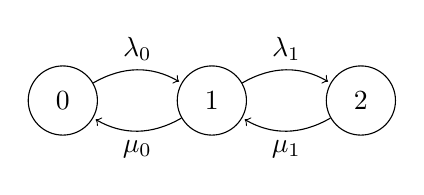
\begin{tikzpicture}
	% Draw the states
	\node[state]             (1) {$0$};
	\node[state, right=of 1] (2) {$1$};
	\node[state, right=of 2] (3) {$2$};
    % Connect the states with arrows
	\draw[every loop]
		(1) edge[bend left, auto=left] node {$\lambda_0$} (2)
		(2) edge[bend left, auto=left] node {$\mu_0$} (1)
		(2) edge[bend left, auto=left] node {$\lambda_1$} (3)
		(3) edge[bend left, auto=left] node {$\mu_1$} (2);
\end{tikzpicture} $\cdots$

\end{center}
Entonces $\pi_{i+1}\mu_{i+1} + \pi_{i-1}\lambda_{i-1} = \pi_i (\lambda_i+\mu_i)$. De manera que
$$
\pi_k = \frac{\lambda_0 \cdots \lambda_{k-1}}{\mu_1 \cdots \mu_k } \pi_0
$$

\end{nota}

\begin{defi} Ejemplos de Procesos de Nacimiento y Muerte.
\begin{itemize}
\item \textbf{Proceso de Poisson}. En estos procesos $\lambda_i = \lambda$ y $\mu_i = 0$. A partir de aquí calcular la matriz $G$ es sencillo, pues la supra diagonal es siempre $\lambda$ y la diagonal $-\lambda$. Usando un teorema anterior, podemos calcular los $\rho_t$. Entonces
$$
\rho_0(t)=-\lambda \rho_0 (t)  \Rightarrow \rho_0(t) = ke^{-\lambda t}
$$
La segunda ecuación es
$$
\rho_1'(t) = \lambda \rho_0(t) - \lambda \rho_1(t)
$$
Resolvemos la ecuación homogénea y por método de variación de constantes. Obtenemos, finalmente, $\rho_k(t) = e^{-\lambda t} \frac{(\lambda t)^k}{k!}$. Para ver si es estacionario,
$$
\pi G = 0
$$
Tenemos que $\pi_{i-1} \lambda = \pi_i \lambda$. Por tanto, $\pi_i = c$ $\forall i$. Dado que $\sum \pi_i = 1$ tenemos que no puede existir.
\item \textbf{Proceso de Yule}. En este proceso no hay un caso $0$, empezamos en $1$. En este caso $\mu_i = 0$ y $\lambda_i =i \lambda $. Este proceso también se conoce como nacimiento puro lineal.
\item \textbf{Proceso de muerte pura}. Consideramos $N$ indidividuos con tiempo de vida exponencial con misma tasa de muerte $\mu$. Por tanto, pasamos del estado $N$ a $N-1$ con tasa $N\mu$. De $N-1$ a $N-2$ con $(N-1)\mu$ y así.
$$
P[X(t)=k] = \binom{N}{k}e^{-k\mu t} (1-e^{-\mu t})^N
$$
\item \textbf{Proceso de inmigración y muerte pura}. La población crece desde $0$ con tasa $\lambda$ y mueren con $\mu_i = i \mu$.
\item Existe otro proceso donde $\lambda_i = \lambda$ y $\mu_i = \mu$.

\end{itemize}
\end{defi}
\end{document}
